\section{行事予定}
\begin{itemize}
\item 後期授業開始
10月1日(木)$\sim$
\item 第55回工大祭
11月21日(土)$\sim$11月22日(日)
\item トマトロボット競技会
12月18日$\sim$20日(金$\cdot$土$\cdot$日)
\end{itemize}

\section{今のところ(9月)の決定事項は}
アーム$\cdots$ハサミ。糸を巻き取ることで切断する\\
機構$\cdots$仮にアームのものを作成することに決めた。\\
センサー$\cdots$キネクトもしくは、ステレオカメラを希望\\
カメラとPSDセンサ(距離センサ)を使用する案もあります。\\
\section{現状}
開発が遅れに遅れている状態ではあるが、未だに大会までに時間を感じている状態にあるが、それは曖昧すぎて現実味が感じられないからである。実際はとてもやばいです。

\section{9月7日の西田先生との話し合いのまとめ}
部品の選定は以下のページを参考にすること
\begin{itemize}
\item ロボット王国
\item 共立エレショップ
\end{itemize}

当初の考えは、ボールねじを用いた超精密駆動が実現できるものであったが、たわみ等バランスを考えると、ネジが回らないとの指摘を受けました。
価格のこともあり、久しぶりにarcの現状を見て、なんか進んでないな$\sim$と正直思いました。

CADをして設計を早く完成させよう、という話でしたが、個人的な意見としては、もうCADをするよりも手で大まかに計算して作り始める方が良いのではないかと思います。

バランスのとれた設計とすること。
ゆっくり動くロボットを作ってもダメ。見ていて面白いものでなければ。

という方針でした。

いずれにしても。

\section{方針}
Raspberry Pi を使用して、土台を動かす\\
Raspberry Pi を使用して、アームを動かす\\
Kinect はPCに接続
PCがRaspberry Piに信号を送信する。

計画が建てられない状況ですので、とりあえず今日はセンサを動かしてトマトを認識してみよう。

\begin{figure}[htbp]
\begin{center}
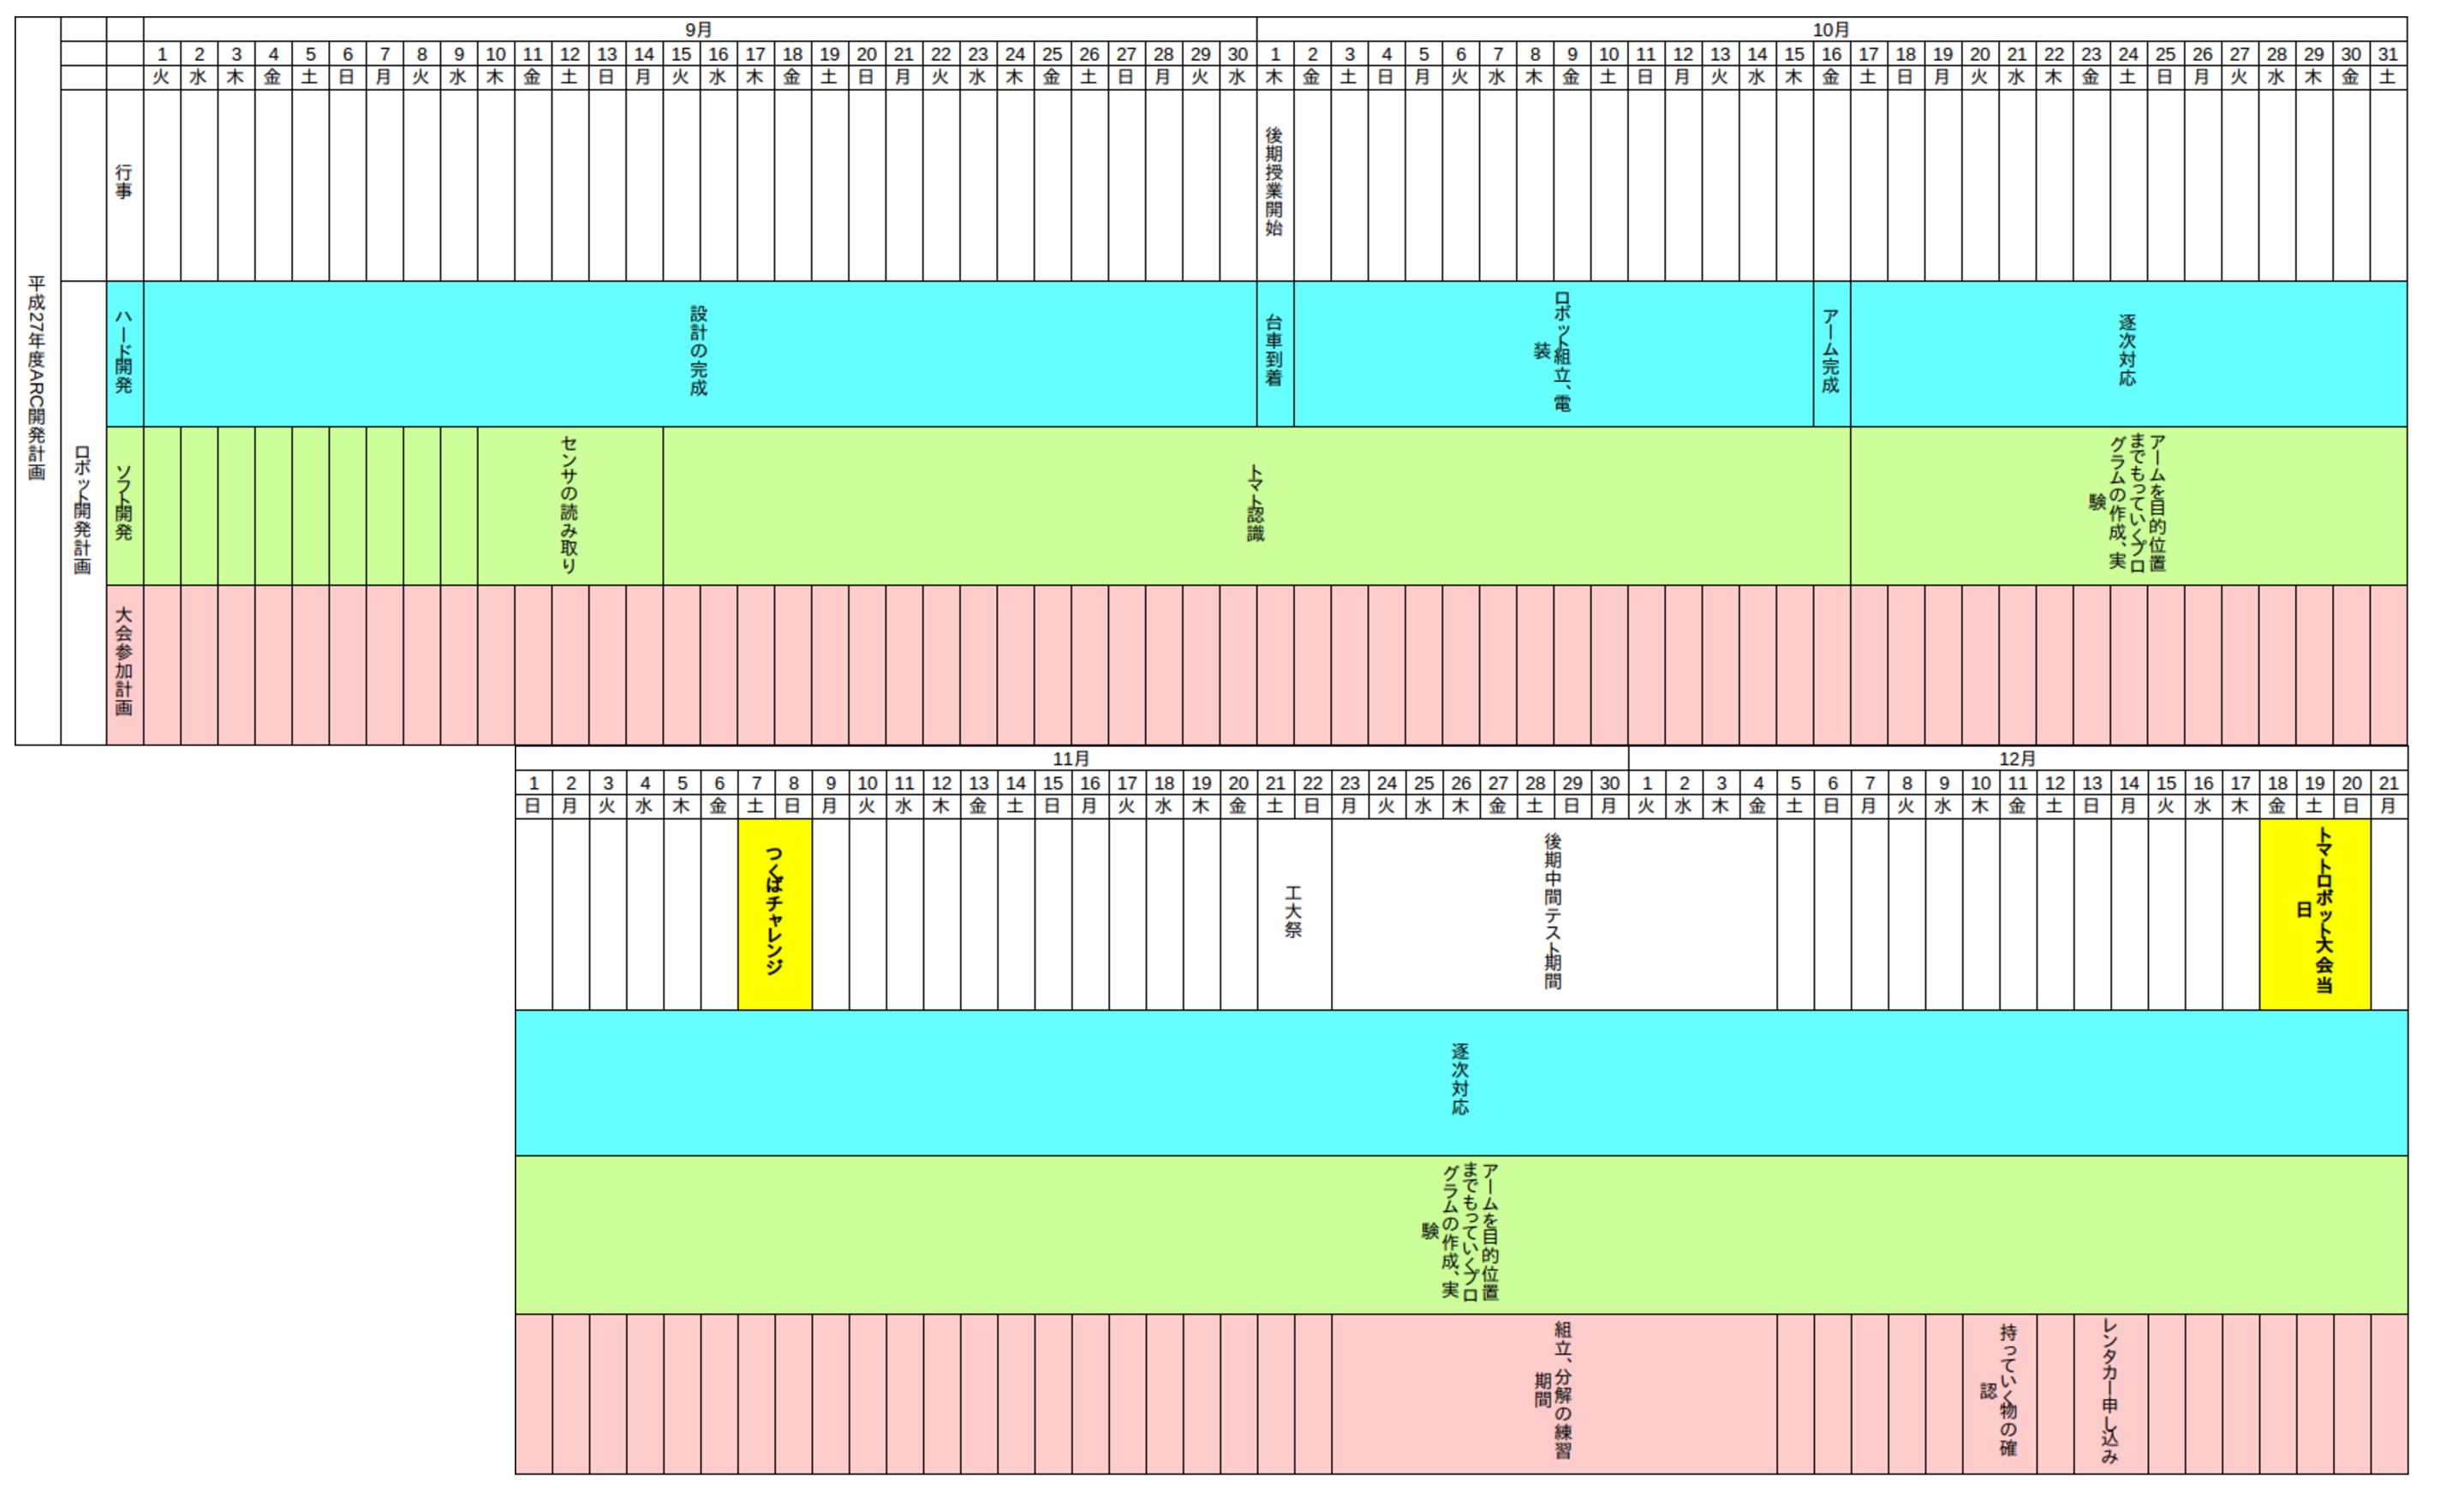
\includegraphics[width=25cm,angle=90]{../arc_plan.eps}
\end{center}
\caption{予定}
\end{figure}
